\chapter{Experimentación: modelos, \\entrenamiento y generación}

En este capítulo usaremos todos los conceptos vistos en los capítulos anteriores para justificar las elecciones de los diferentes modelos, hablaremos de las características principales de los mismos y finalmente entraremos en la fase del entrenamiento y los resultados de dichos modelos.





\section{EDA y preprocesamiento}

En esta sección expondremos los diferentes métodos y técnicas utilizadas de preprocesamiento de texto para darle una forma apropiada y unificada al conjunto de datos, antes de poder introducirlos en el modelo.

En la Figura \ref{fig:preprocess-diagram} se ilustra un esquema de los pasos a seguir en esta fase del proyecto. Explicaremos cada paso desde el punto de vista de los dos conjuntos de datos a unificar, ya que cada uno necesitará de un tratamiento particular en función de su etado inicial.

\begin{figure}[h!]
	\centering
	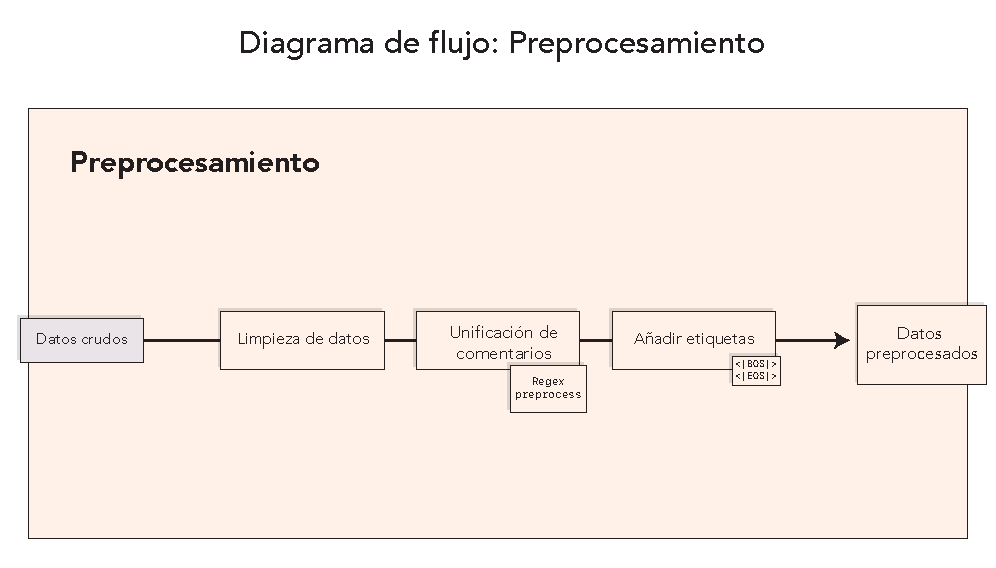
\includegraphics[width=.9\textwidth]{media/preprocess-diagram.pdf}
	\caption{Diagrama resumen del preprocesamiento efectuado en los datos.}
	\label{fig:preprocess-diagram}
\end{figure}


\subsection{Datos: fuente y forma}
Los datos escogidos provienen del dataset \href{https://www.kaggle.com/chaitanyakck/medical-text}{Medical Text} publicado por Chaitanya Krishna Kasaraneni, y de \href{https://www.kaggle.com/tboyle10/medicaltranscriptions}{Medical Transcriptions}, publicado por Tara Boyle. La naturaleza de los mismos es ligeramente diferente así que explicaremos el proceso de preprocesamiento y unificación posteriormente.

En la Figura \ref{fig:preprocess-diagram} podemos ver un pequeño resumen del preprocesamiento que se acometerá a los datos. En la siguiente sección se detallan cada uno de estos pasos.

\subsubsection{Dataset: \textit{Medical Text}}
El dataset tiene formato \jesitt{.dat}, estructurado como un \jesitt{.tsv} (Tab Separated Values). La primera columna corresponde con una categoría determinada --ya que el dataset estaba diseñado para clasificación-- y la segunda columna contiene fragmentos de documentos médicos.

El dataset es en inglés, está anonimizado y los comentarios principalmente consisten en descripciones quirúrjicas o relacionadas con operaciones complejas. Podemos ver los dos primeros de nuestro conjunto de datos en los Comentarios \ref{com:com1} y \ref{com:com2}.

\begin{thm}
	\sffamily{
		Excision of limbal dermoids. We reviewed the clinical files of 10 patients who had undergone excision of unilateral epibulbar limbal dermoids. Preoperatively, all of the affected eyes had worse visual acuity (P less than .02) and more astigmatism (P less than .01) than the contralateral eyes. Postoperatively, every patient was cosmetically improved. Of the eight patients for whom both preoperative and postoperative visual acuity measurements had been obtained, in six it had changed minimally (less than or equal to 1 line), and in two it had improved (less than or equal to 2 lines). Surgical complications included persistent epithelial defects (40\%) and peripheral corneal vascularization and opacity (70\%). These complications do not outweigh the cosmetic and visual benefits of dermoid excision in selected patients. 
	}
	\label{com:com1}
\end{thm}
\begin{thm}
	\sffamily{
		Retained endobronchial foreign body removal facilitated by steroid therapy of an obstructing, inflammatory polyp. Oral and topical steroids were used to induce regression in an inflammatory, obstructing endobronchial polyp caused by a retained foreign body. The FB (a peanut half), which had been present for over six months, was then able to be easily and bloodlessly retrieved with fiberoptic bronchoscopy. 
	}
	\label{com:com2}
\end{thm}

El dataset está descompuesto en un archivo \jesitt{train.dat} y otro \jesitt{test.dat}. El archivo de entrenamiento contiene 14438 comentarios, y el de evaluación, 14442. En total, disponemos de 28880 comentarios.

\subsubsection{Análisis de datos exploratorio}
En esta subsección, analizaremos en más profundidad la forma de los datos, para saber qué esperar de cara al entrenamiento de nuestros modelos.

Como podemos observar en las figuras \ref{fig:avg_char_train} y \ref{fig:avg_tokens_train}, la distribución de los distintos elementos de nuestro dataset de entrenamiento está muy normalmente distribuída.

El número medio de caracteres por comentario es de 1230, y el número medio de tokens por comentario es de unos 180, correspondiéndose con las líneas amarillas en las figuras.

Se pueden apreciar, aún así, algunos valores atípicos de comentarios particularmente largos. Esto, sin embargo, no es necesariamente malo en nuestro caso. En definitiva, cuanto más texto tengamos a nuestra disposición, mejor para el modelo.

\begin{figure}[h!]
	\centering
	\begin{subfigure}[t]{0.95\textwidth}
		\centering
		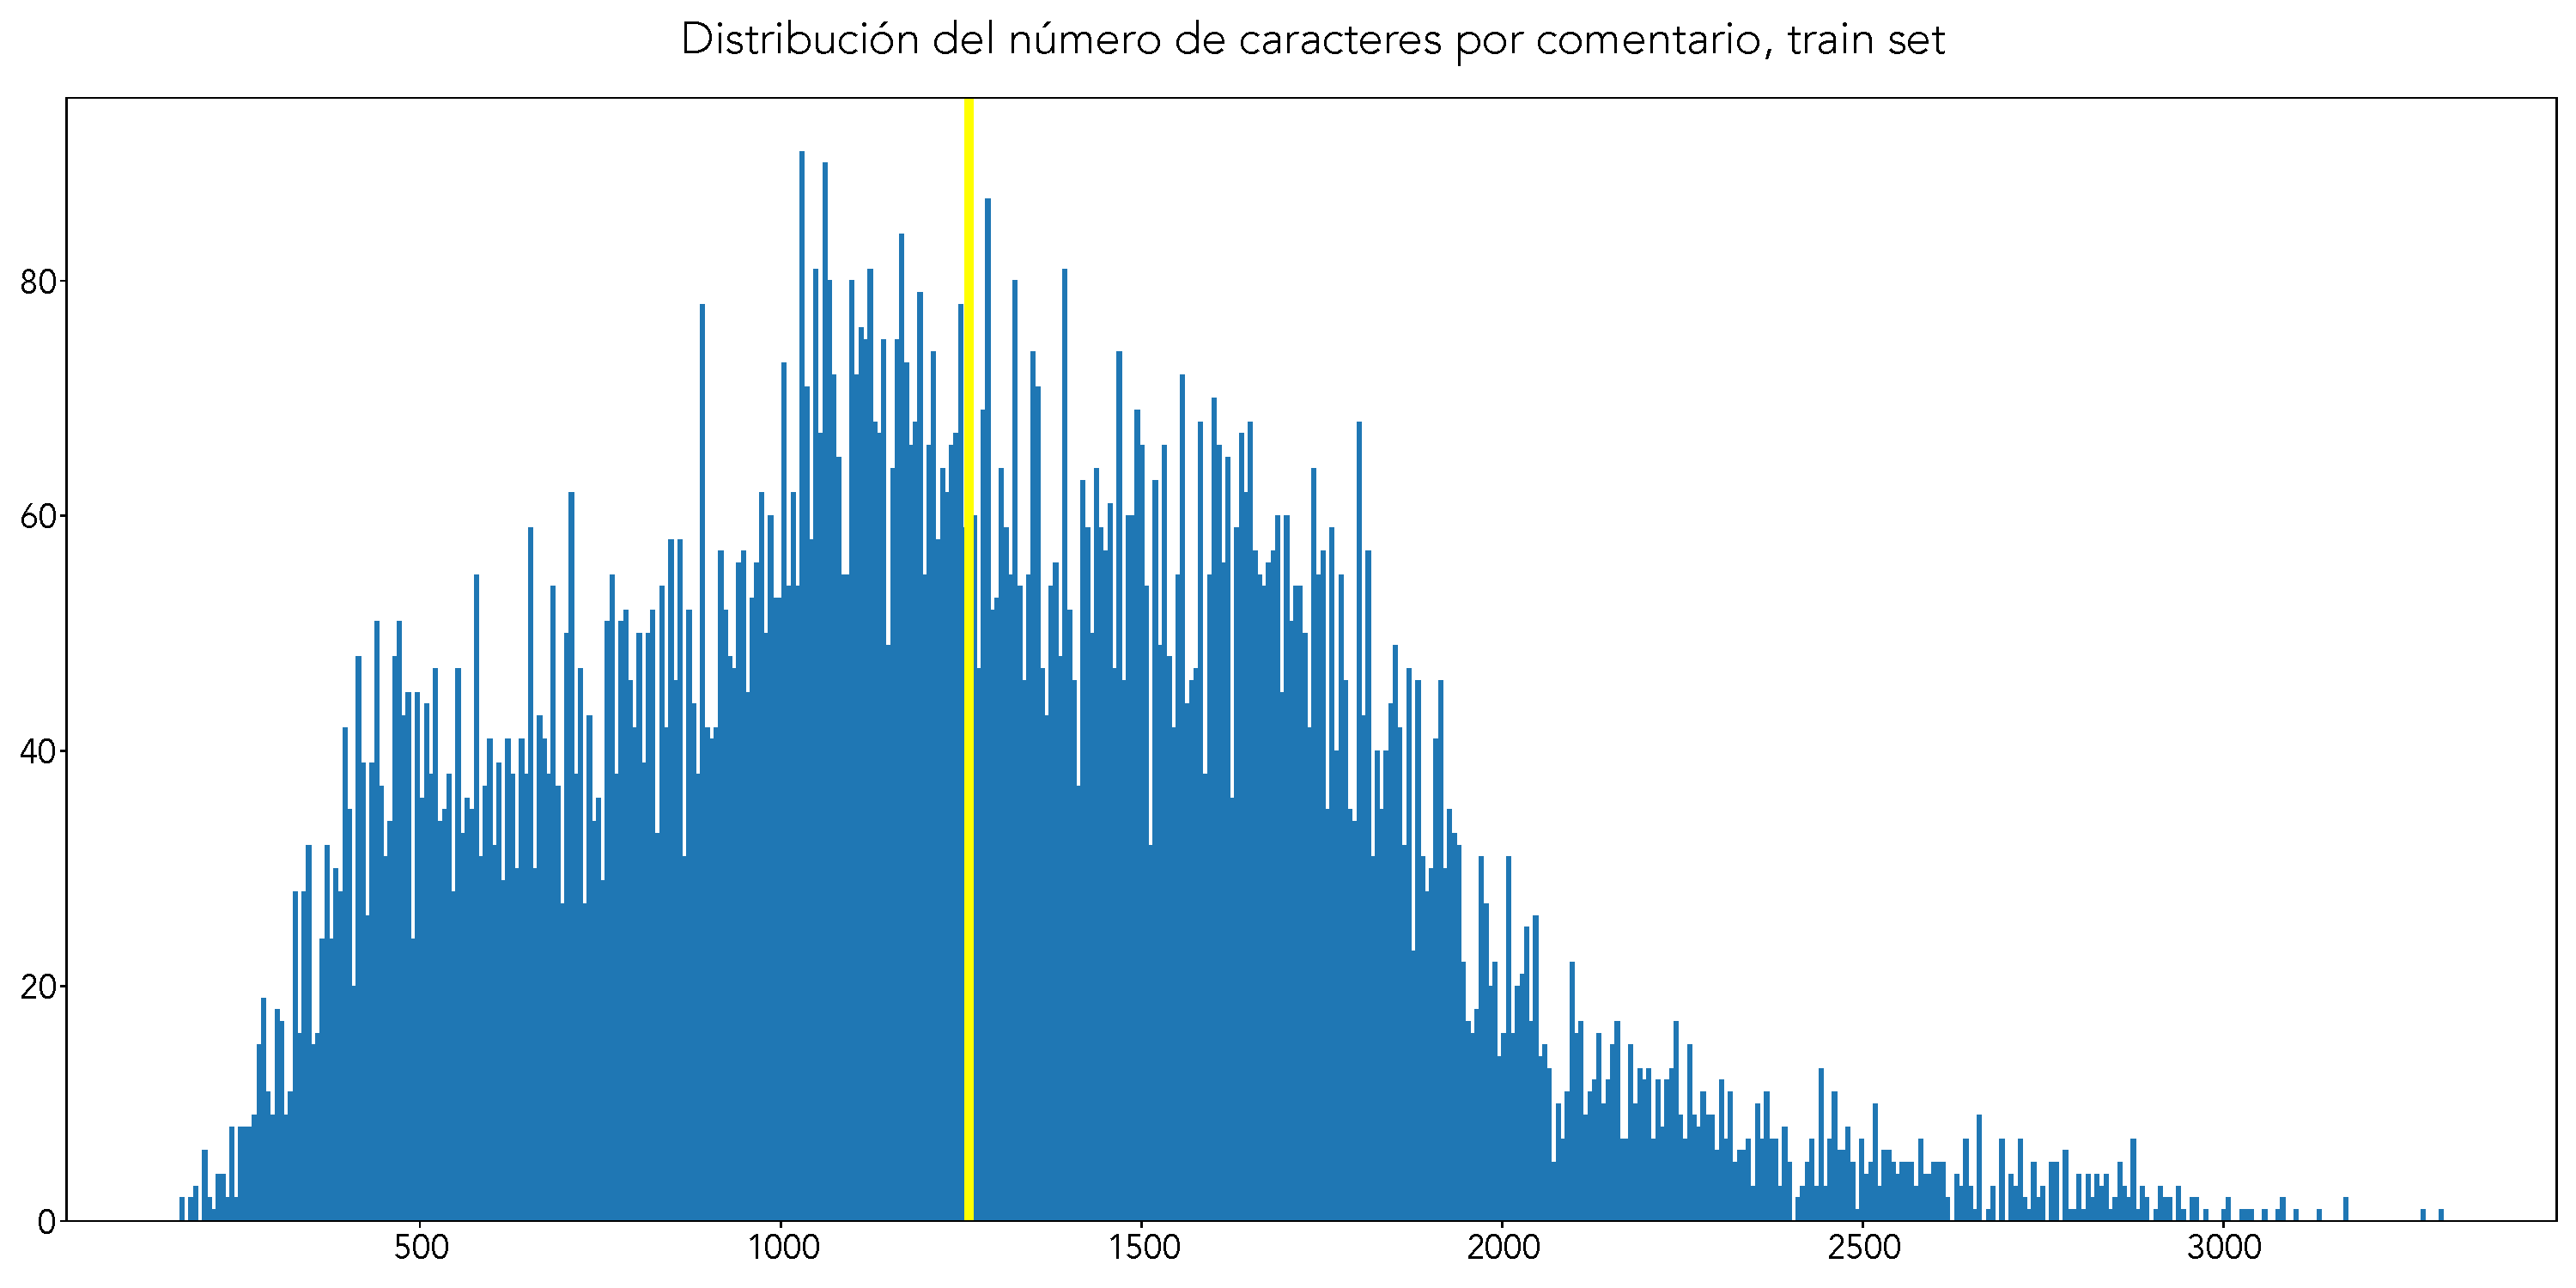
\includegraphics[width=.9\textwidth]{media/char_hist_train.pdf}
		\caption{Distribución del número de caracteres por comentario, en el conjunto de entrenamiento}
		\label{fig:avg_char_train}
	\end{subfigure}
	~

	\begin{subfigure}[t]{0.95\textwidth}
		\centering
		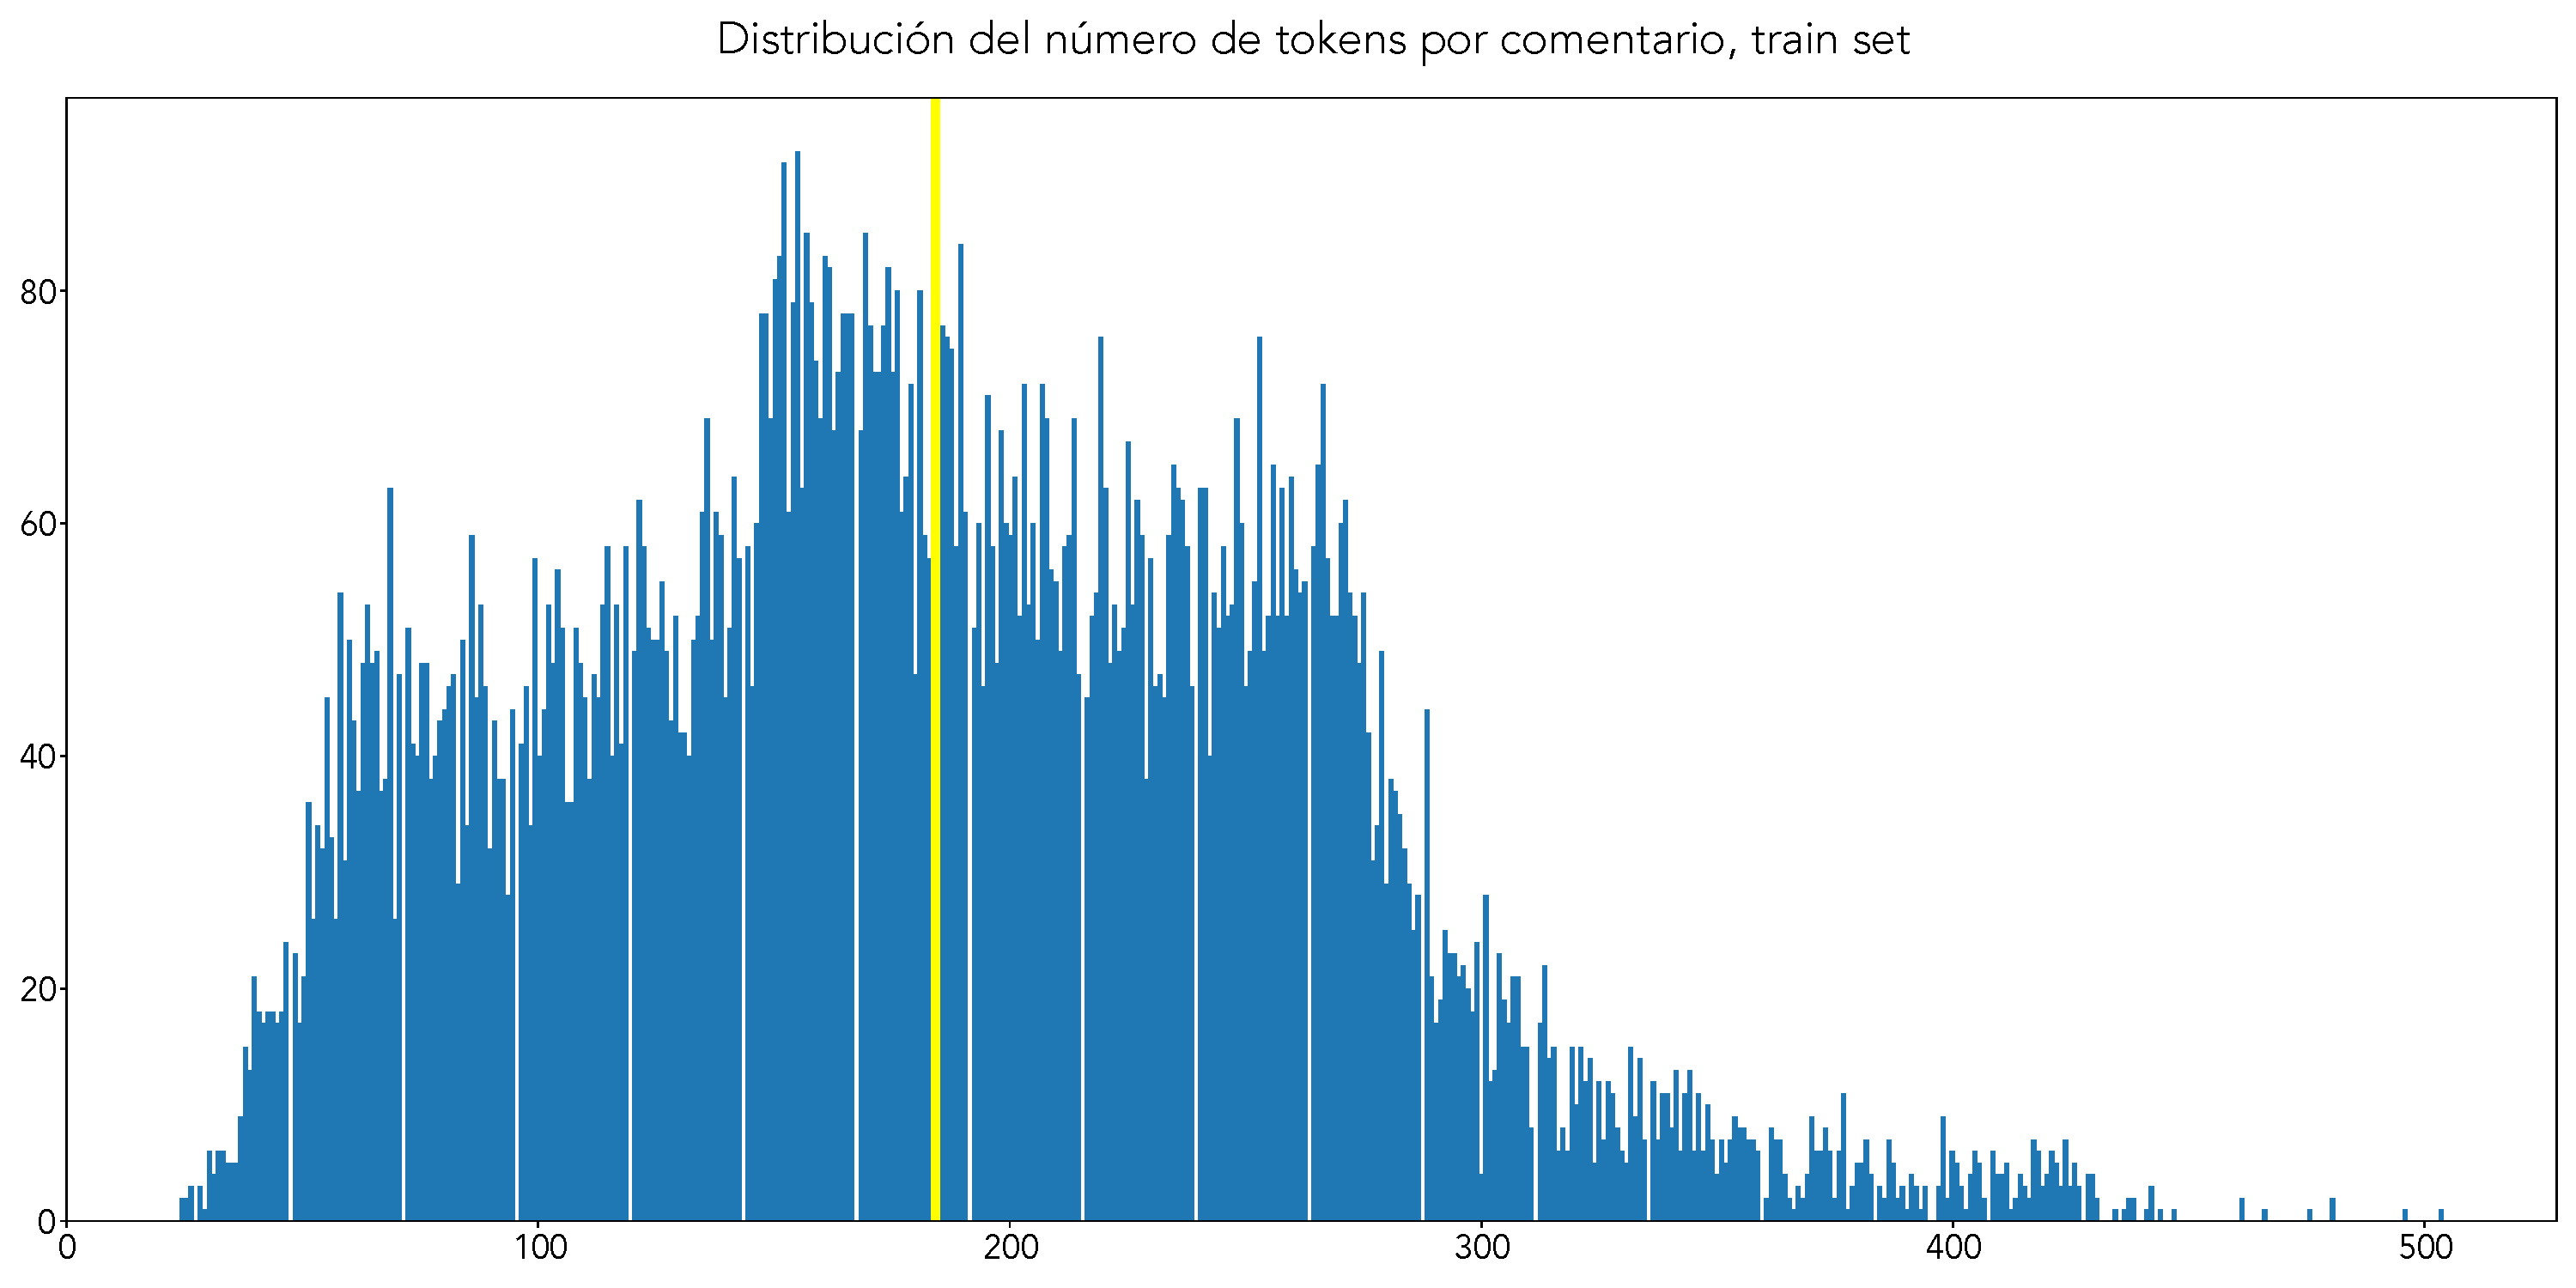
\includegraphics[width=.9\textwidth]{media/tokens_hist_train.pdf}
		\caption{Distribución del número de tokens por comentario en el conjunto de entrenamiento}
		\label{fig:avg_tokens_train}
	\end{subfigure}

	\caption{Visualización de la distribución de nuestro conjunto de entrenamiento}
	\label{fig:sum_train}
\end{figure}


\begin{figure}[h!]
	\centering
	\begin{subfigure}[t]{0.95\textwidth}
		\centering
		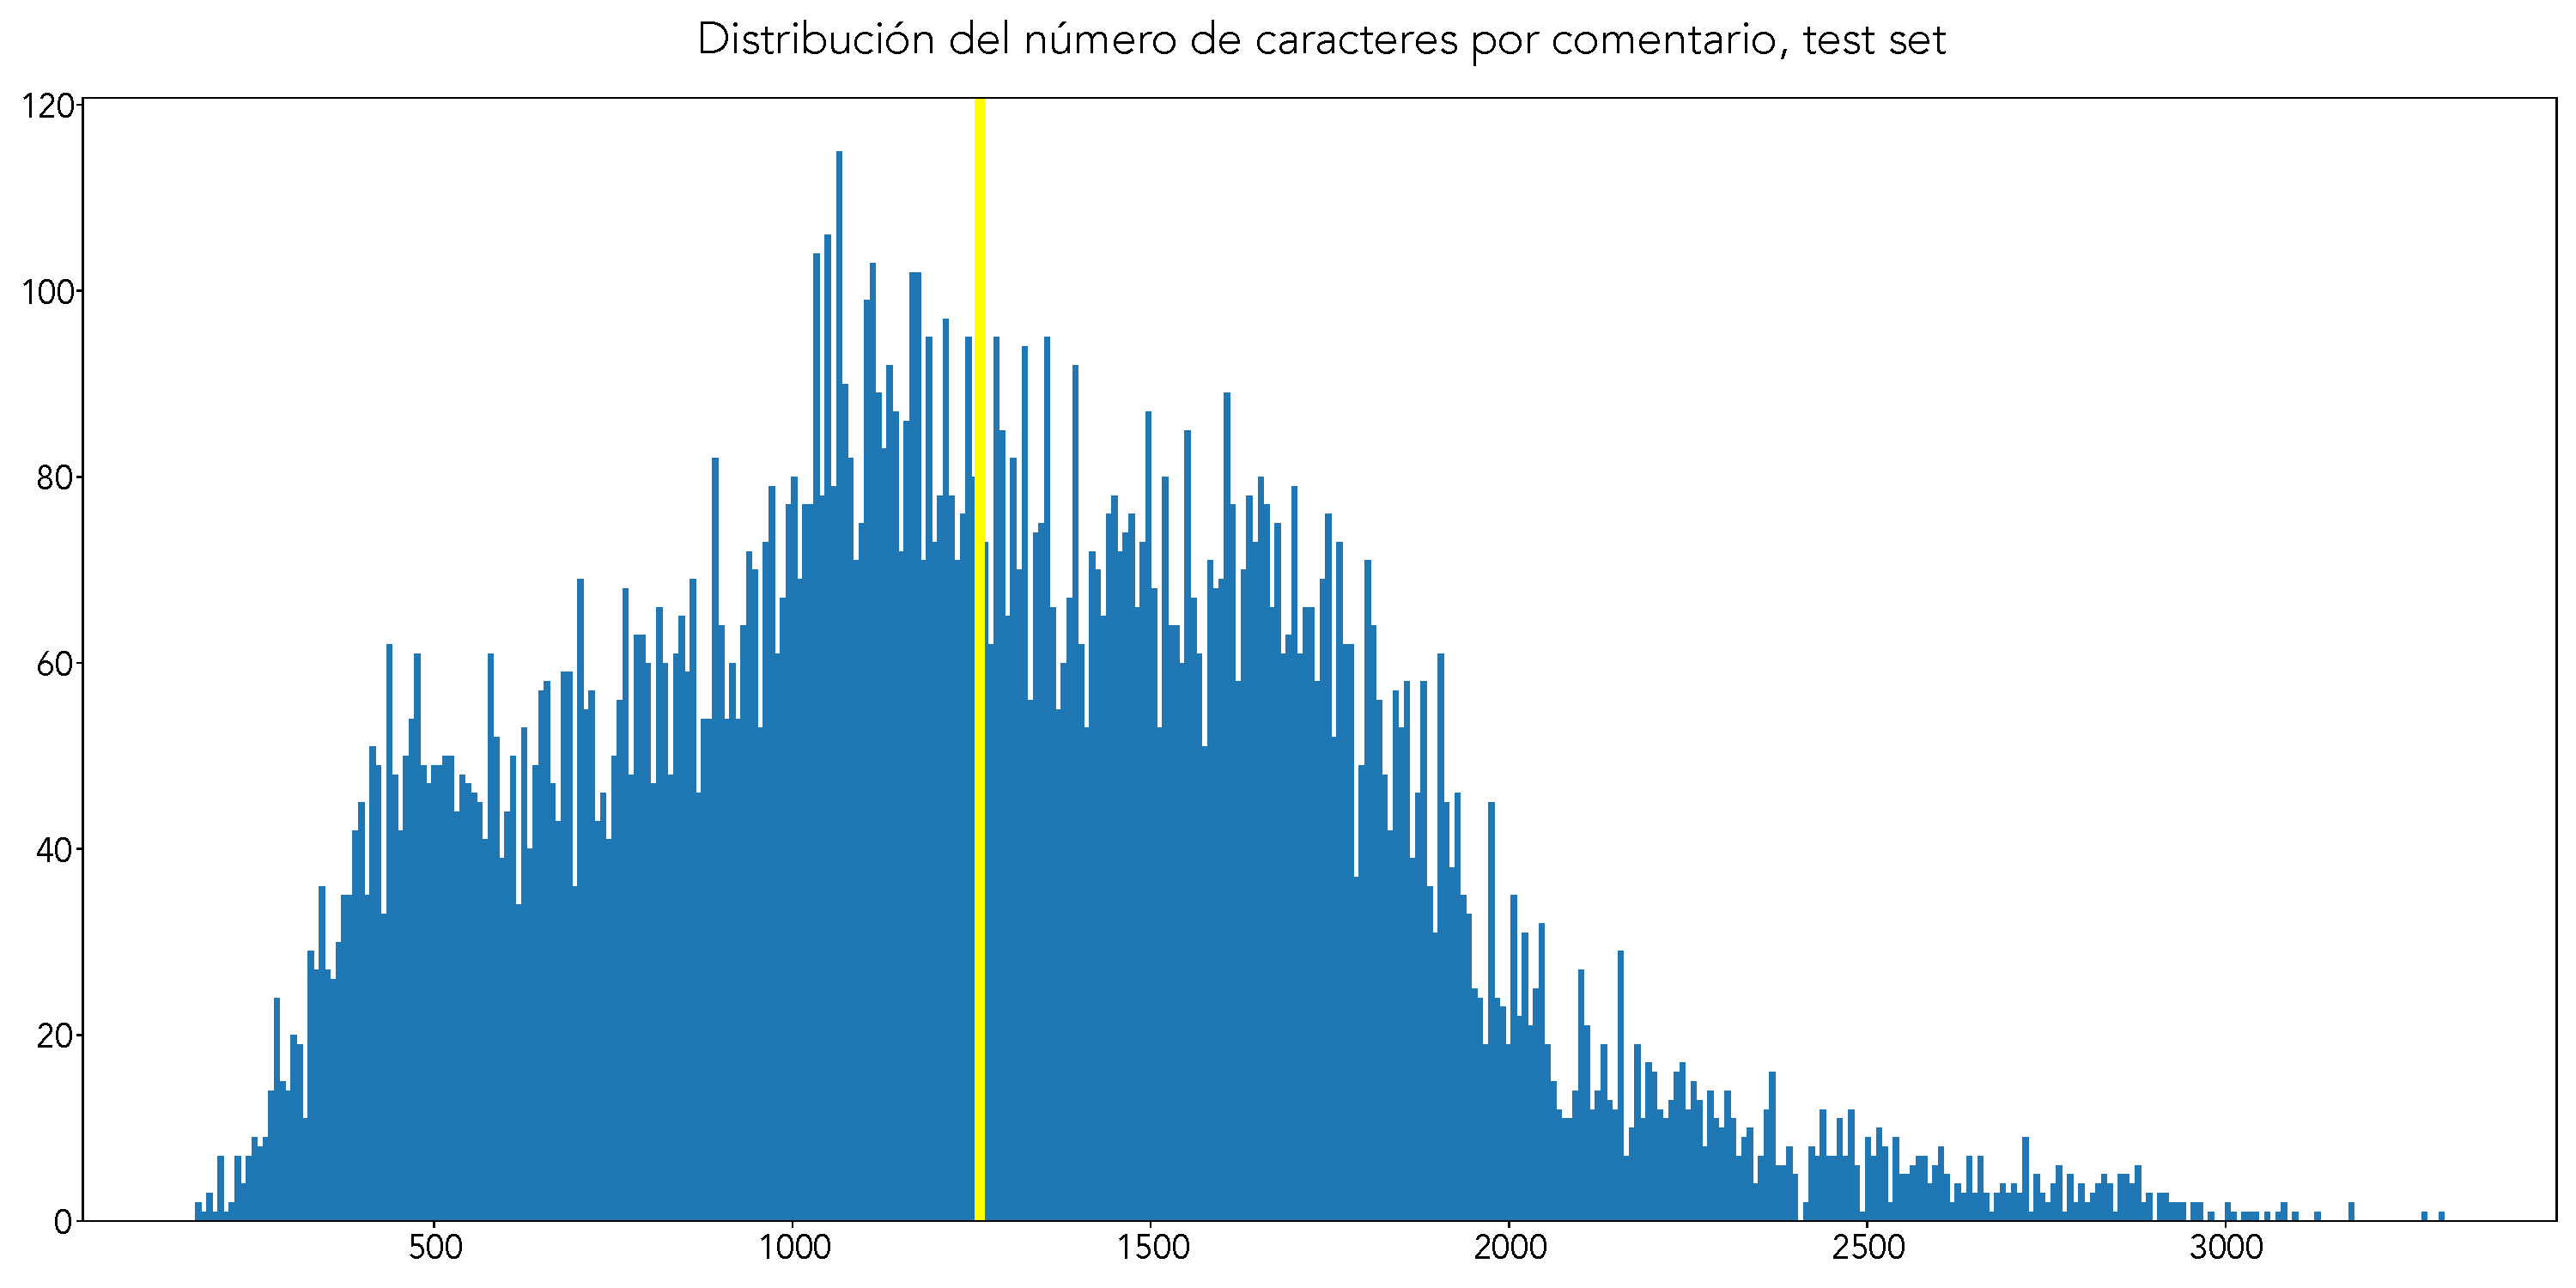
\includegraphics[width=.9\textwidth]{media/char_hist_test.pdf}
		\caption{Distribución del número de caracteres por comentario, en el conjunto de evaluación}
		\label{fig:avg_char_test_test}
	\end{subfigure}

	~

	\begin{subfigure}[t]{0.95\textwidth}
		\centering
		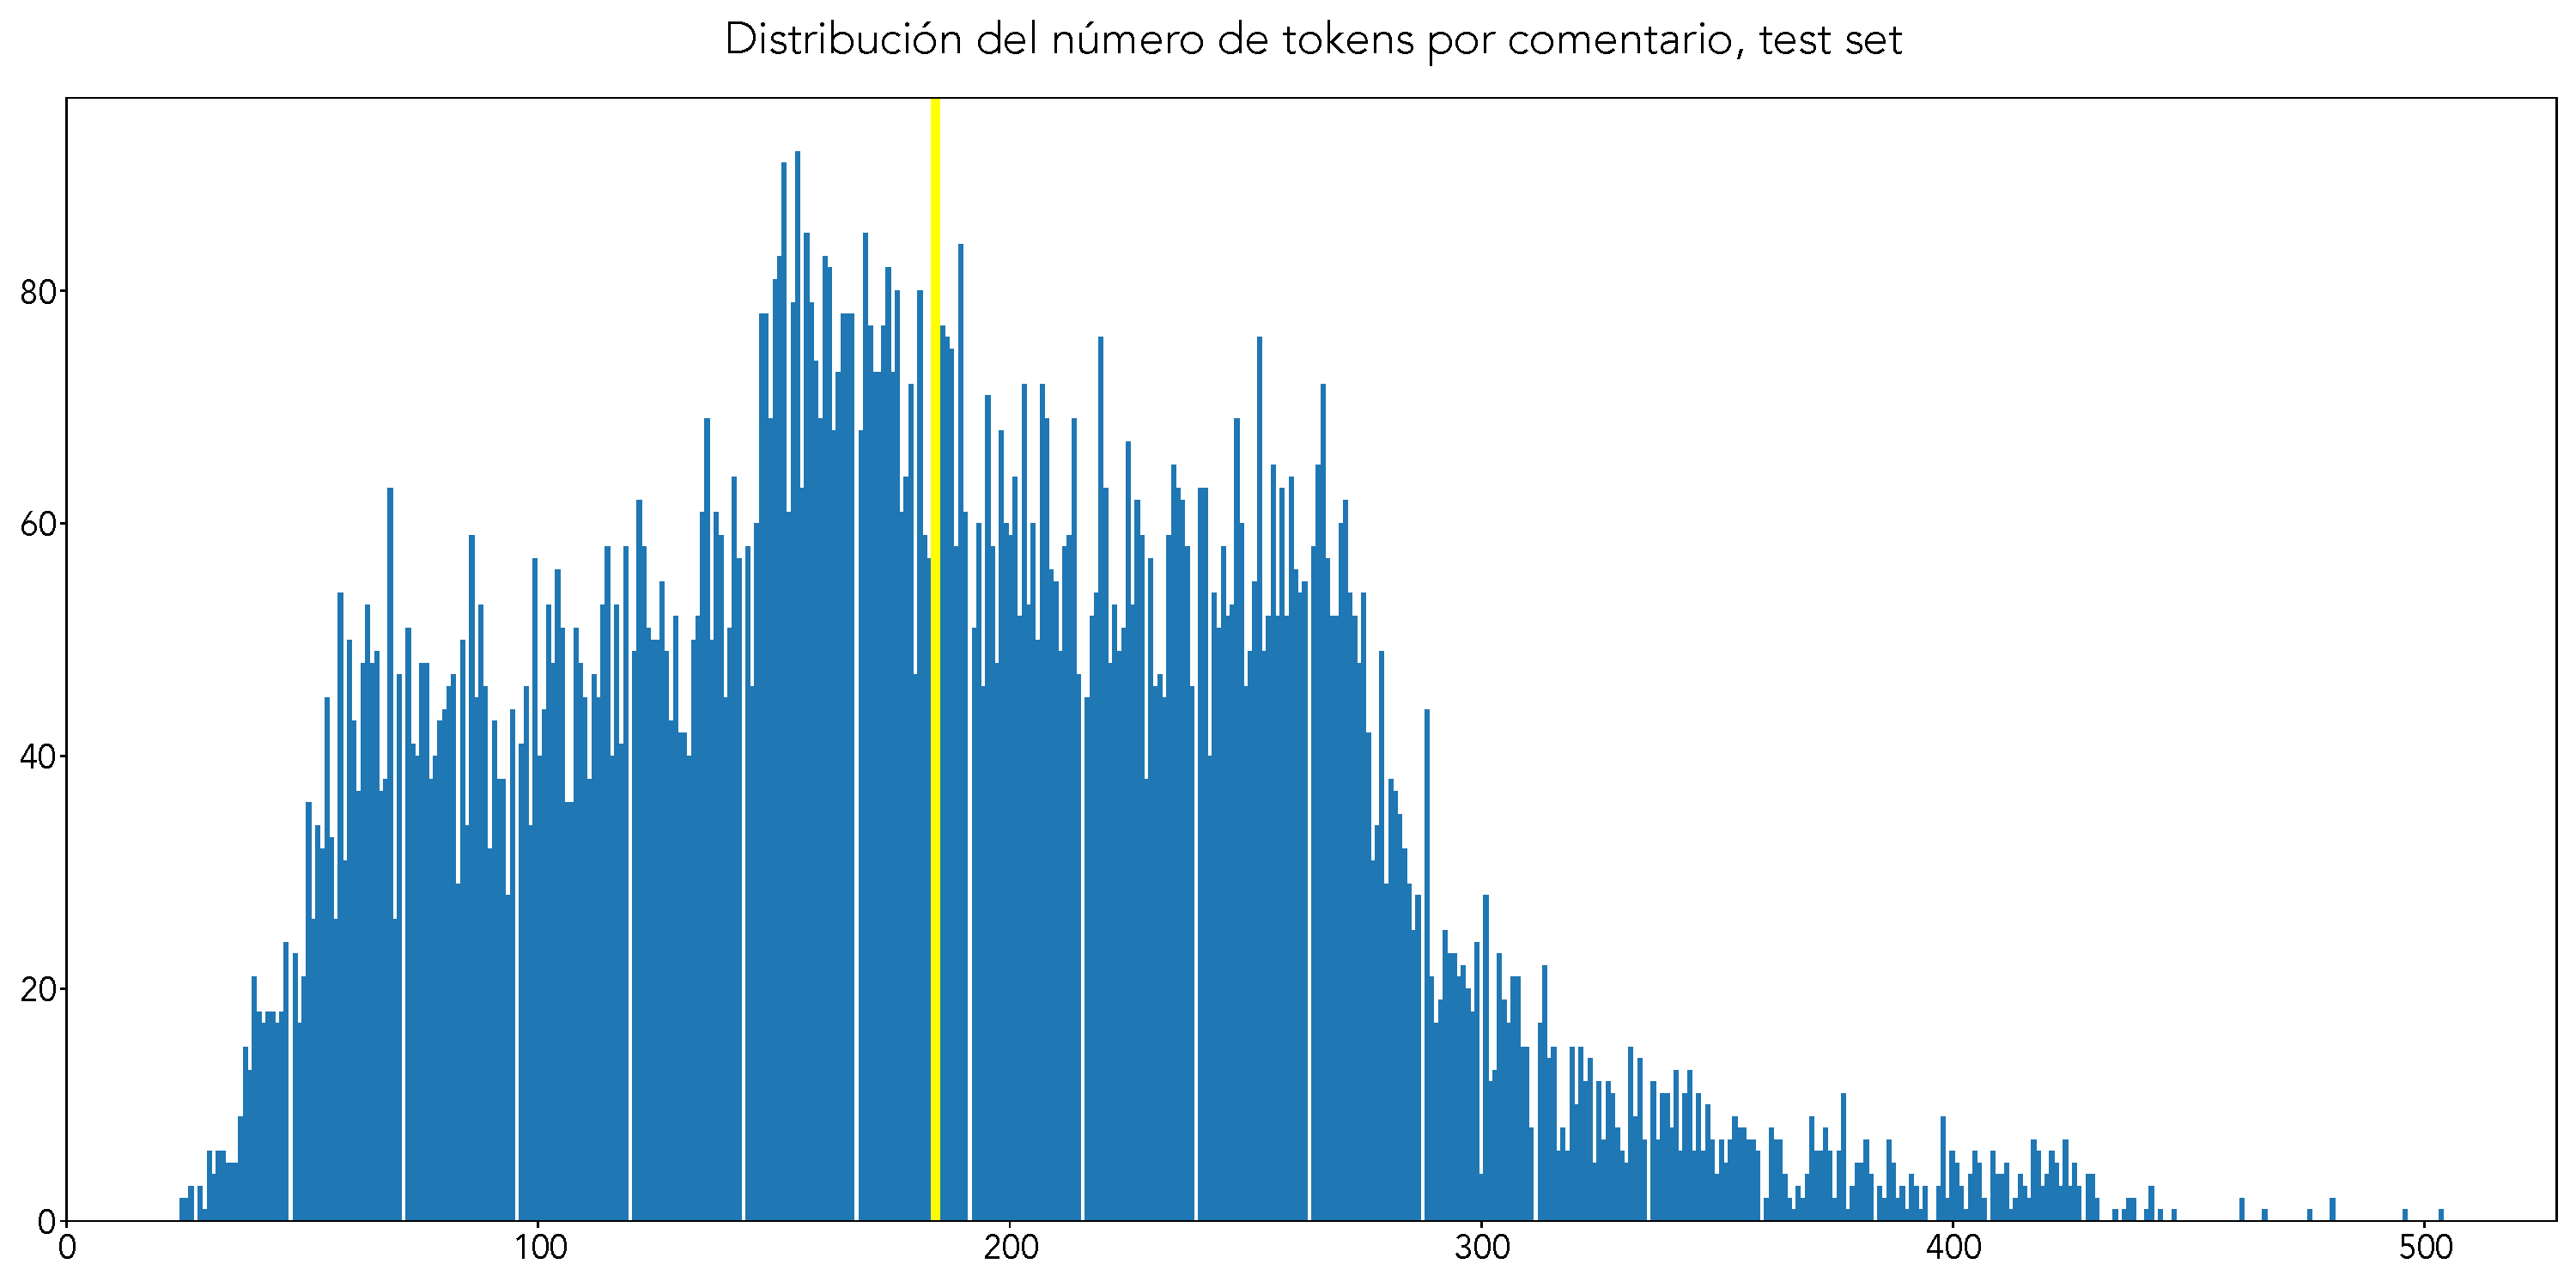
\includegraphics[width=.9\textwidth]{media/tokens_hist_test.pdf}
		\caption{Distribución del número de tokens por comentario en el conjunto de evaluación}
		\label{fig:avg_tokens_test}
	\end{subfigure}


	\caption{Visualización de la distribución de nuestro conjunto de evaluación}
	\label{fig:sum_test}
\end{figure}

Una media de casi 200 palabras por comentario con comentarios alcanzando las 500 corresponde con comentarios relativamente largos. Esto nos vendrá bien de cara al entrenamiento de nuestro modelo, para poder formar oraciones con más sentido.


\subsubsection{Dataset: \textit{Medical Transcriptions}}
Este dataset es en realidad una extracción de la página web \url{mtsamples.com}, donde se halla una respetable cantidad de trasncripciones médicas. La autora extrajo todos los comentarios, así como los diferentes metadatos que los acompañaban mediante \textit{web scraping} y los provee en la columna \jesitt{trasncription}.

Al igual que el anterior, este conjunto de datos se corresponde con informes de operaciones quirúrjicas en inglés, y de igual forma anonimizado.

En este caso, como podemos apreciar en la Figura \ref{fig:sum_mdtr}, las distribuciones son ligeramente asimétricas, predominando comentarios más cortos. Aún así, disponemos de comentarios excepcionalmente largos, con alrededor de 18000 caracteres.

\begin{figure}[h!]
	\centering
	\begin{subfigure}[t]{0.95\textwidth}
		\centering
		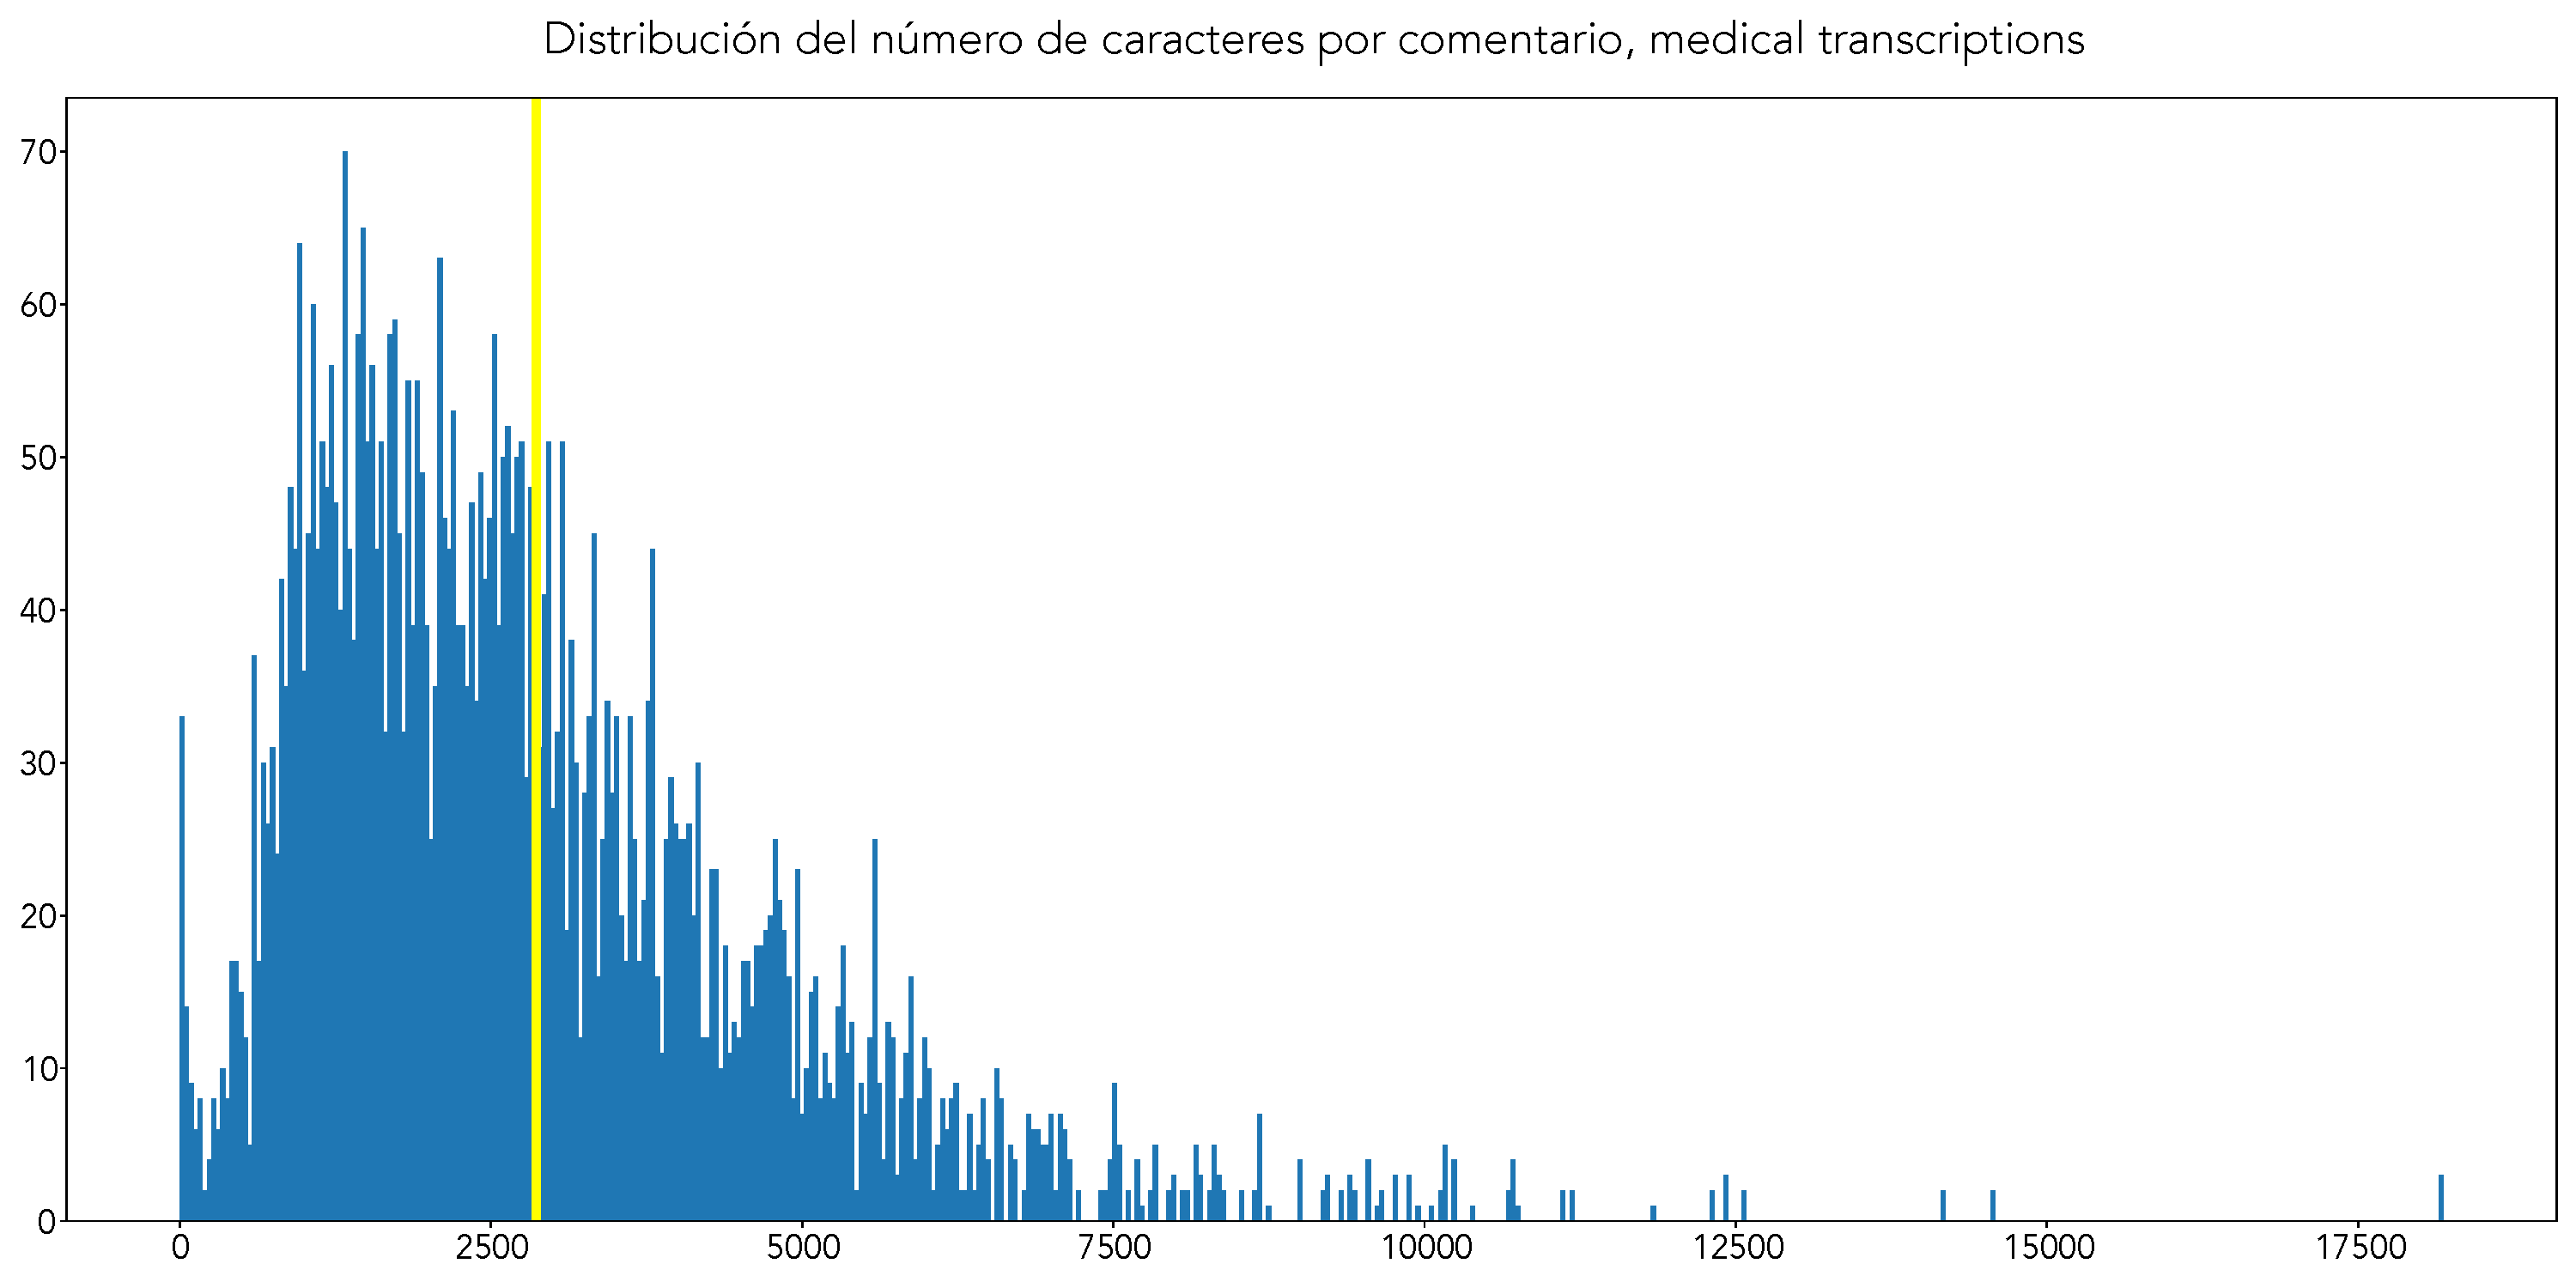
\includegraphics[width=.9\textwidth]{media/char_hist_mdtr.pdf}
		\caption{Distribución de caracteres en el dataset Medical Transcriptions}
		\label{fig:char_hist_mdtr}
	\end{subfigure}

	~
	\begin{subfigure}[t]{0.95\textwidth}
		\centering
		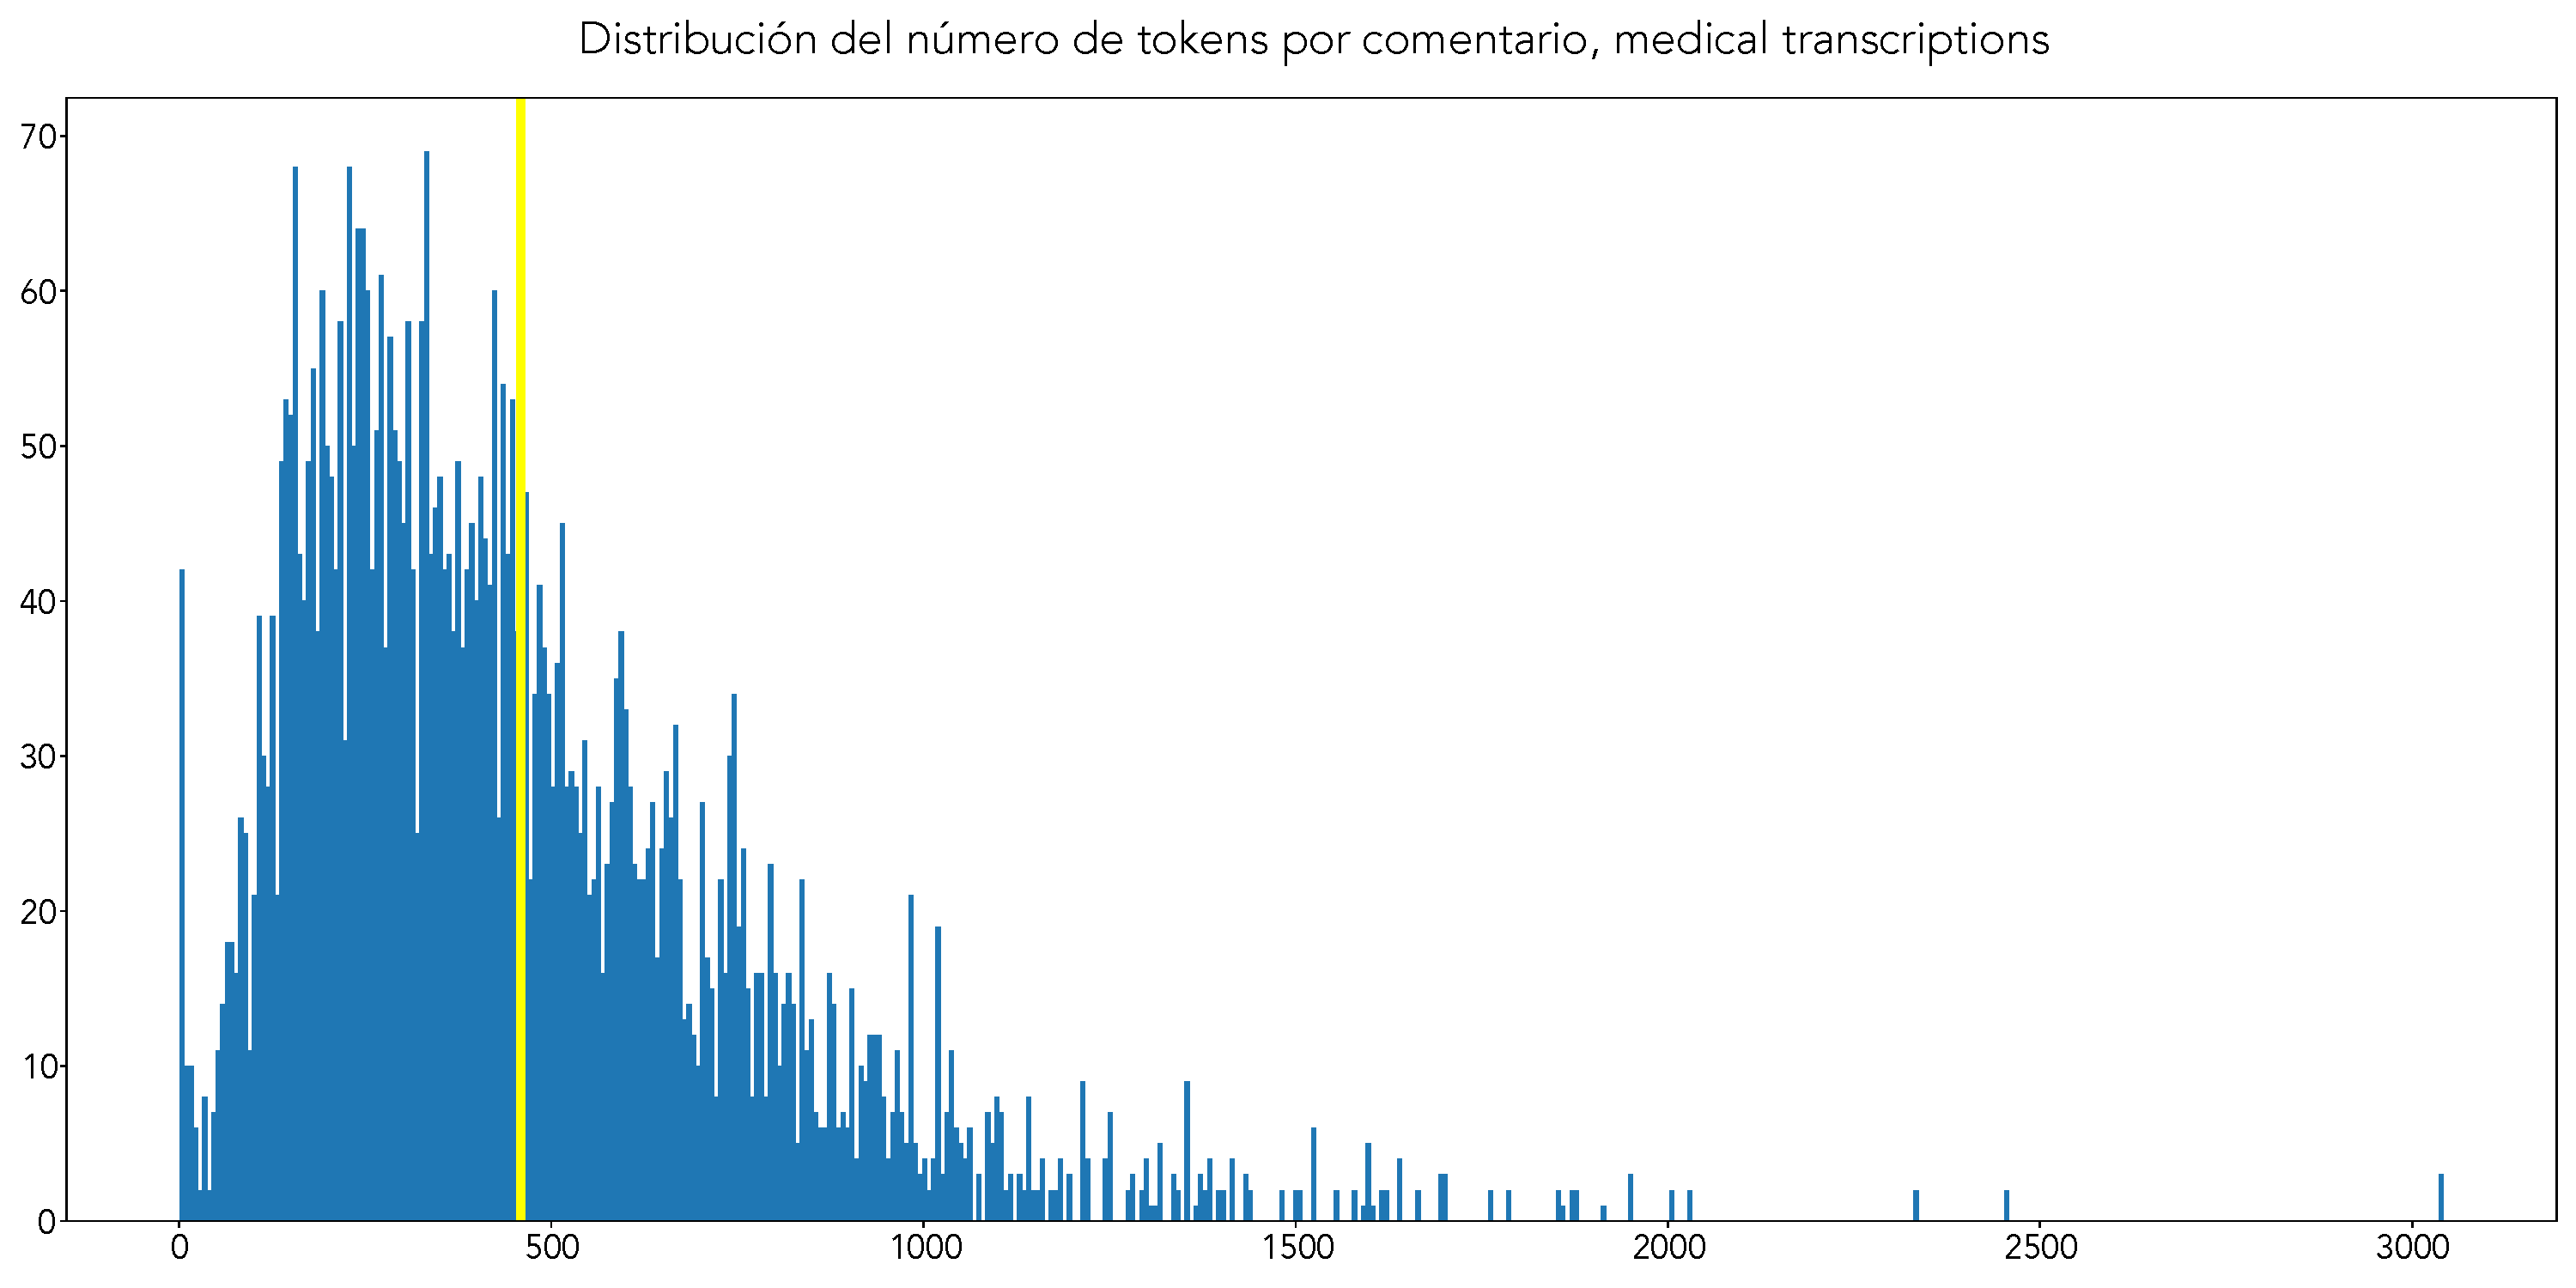
\includegraphics[width=.9\textwidth]{media/token_hist_mdtr.pdf}
		\caption{Distribución de palabras en el dataset Medical Transcriptions}
		\label{fig:token_hist_mdtr}
	\end{subfigure}

	\caption{Visualización del dataset Medical Transcriptions}
	\label{fig:sum_mdtr}
\end{figure}



\subsection{Preprocesamiento}
En esta sección, describiremos el preprocesamiento acometido en cada uno de los datsets. Provienen de fuentes diferentes así que cada uno recibirá un trato diferente, con objeto de normalizar y unificar el formato de todos de cara al entrenamiento.




\subsubsection{Medical Text}
Este conjunto de datos, siendo específicamente texto, el formato, ortografía y en general formato de los archivos es muy bueno. Simplemente hemos de eliminar las categorías adjuntas a cada comentario, para obtener una lista de comentarios crudos en sí. Por lo demás, los comentarios carecen de problemas de formato, codificación o cualquier otra cosa que pudiera interferir con el proceso de entrenamiento. Probablemente el autor ya hiciera esto por nosotros antes de publicarlo.


\subsubsection{Medical Transcriptions}
En el caso de las trancripciones médicas, la tarea es considerablemente más compleja. El conjunto de datos proviene de la página web \url{mtsamples.com}, como especificamos anteriomente. La autora efectuó un proceso de \textit{web scraping} para obtener toda la información y recogerla en el archivo \jesitt{.csv}. 

Esto facilita las cosas, pero desde luego los comentarios deben ser tratados en profundidad antes de poder pasarlos a cualquier modelo. Los trazos de formato en HTML se dejan entrever en los comentarios con signos de puntuación o tabulaciones fuera de lugar, apreciables en el Comentario \ref{com:mt-before}, así que debemos arreglarlo previo entrenamiento.

Para ello, se ha hecho un fuerte uso de expresiones regulares, y se ha creado un \textit{pipeline} para procesar todo el texto a la vez.

El pipeline elimina todas las posibles trazas o residuos que hubieran quedado del \textit{web scraping}. Podemos ver el pipeline diseñado en la Figura \ref{code:pipeline-regex-mdtr} del Apéndice.

El resumen del proceso es eliminar signos de puntuación mal colocados, eliminar títulos o cabeceras de secciones de la página web, sustituir múltiples espacios por uno solo o eliminar los números de listas enumeradas (1., 2., etc). Finalmente, se añaden las etiquetas que vemos en la Figura \ref{fig:preprocess-diagram}. Se explicará su funcionamiento en la sección de la experimentación.

El resultado es un texto muy limpio y claro, mucho más apto para la fase de entrenamiento.

Podemos ver una comparativa del antes (Comentario \ref{com:mt-before}) y el después (Comentario \ref{com:mt-after}) del preprocesamiento de un determinado comentario de nuestro dataset. Los comentarios han sido truncados debido a su longitud.


\begin{thm}
	\sffamily{
		\small{
		SUBJECTIVE:,  This 23-year-old white female presents with complaint of allergies.  She used to have allergies when she lived in Seattle but she thinks they are worse here.  In the past, she has tried Claritin, and Zyrtec.  Both worked for short time but then seemed to lose effectiveness.  She has used Allegra also.  She used that last summer and she began using it again two weeks ago. [...]
		}
	}
	\label{com:mt-before}
\end{thm}


\begin{thm}
	\sffamily{
		\small{
		$<|$ BOS $|>$This 23-year-old white female presents with complaint of allergies. She used to have allergies when she lived in Seattle but she thinks they are worse here. In the past, she has tried Claritin, and Zyrtec. Both worked for short time but then seemed to lose effectiveness. She has used Allegra also. She used that last summer and she began using it again two weeks ago. [...] $<|$ EOS $|>$}
	}
	\label{com:mt-after}
\end{thm}

\subsection{Resultados del preprocesamiento}

Tras haber preprocesado y cribado todos los elementos que pudieran suponer un problema a la hora de entrenar nuestro modelo, lo que obtenemos es un dataset unificado con un total de 33846 comentarios, sumando un total de 7537697 palabras con una media de 222 tokens y 1482 caracteres por comentario. 


Vemos además, en la Figura \ref{fig:wordcloud} una nube de palabras de todo el conjunto de datos.

\begin{figure}[h]
	\centering
	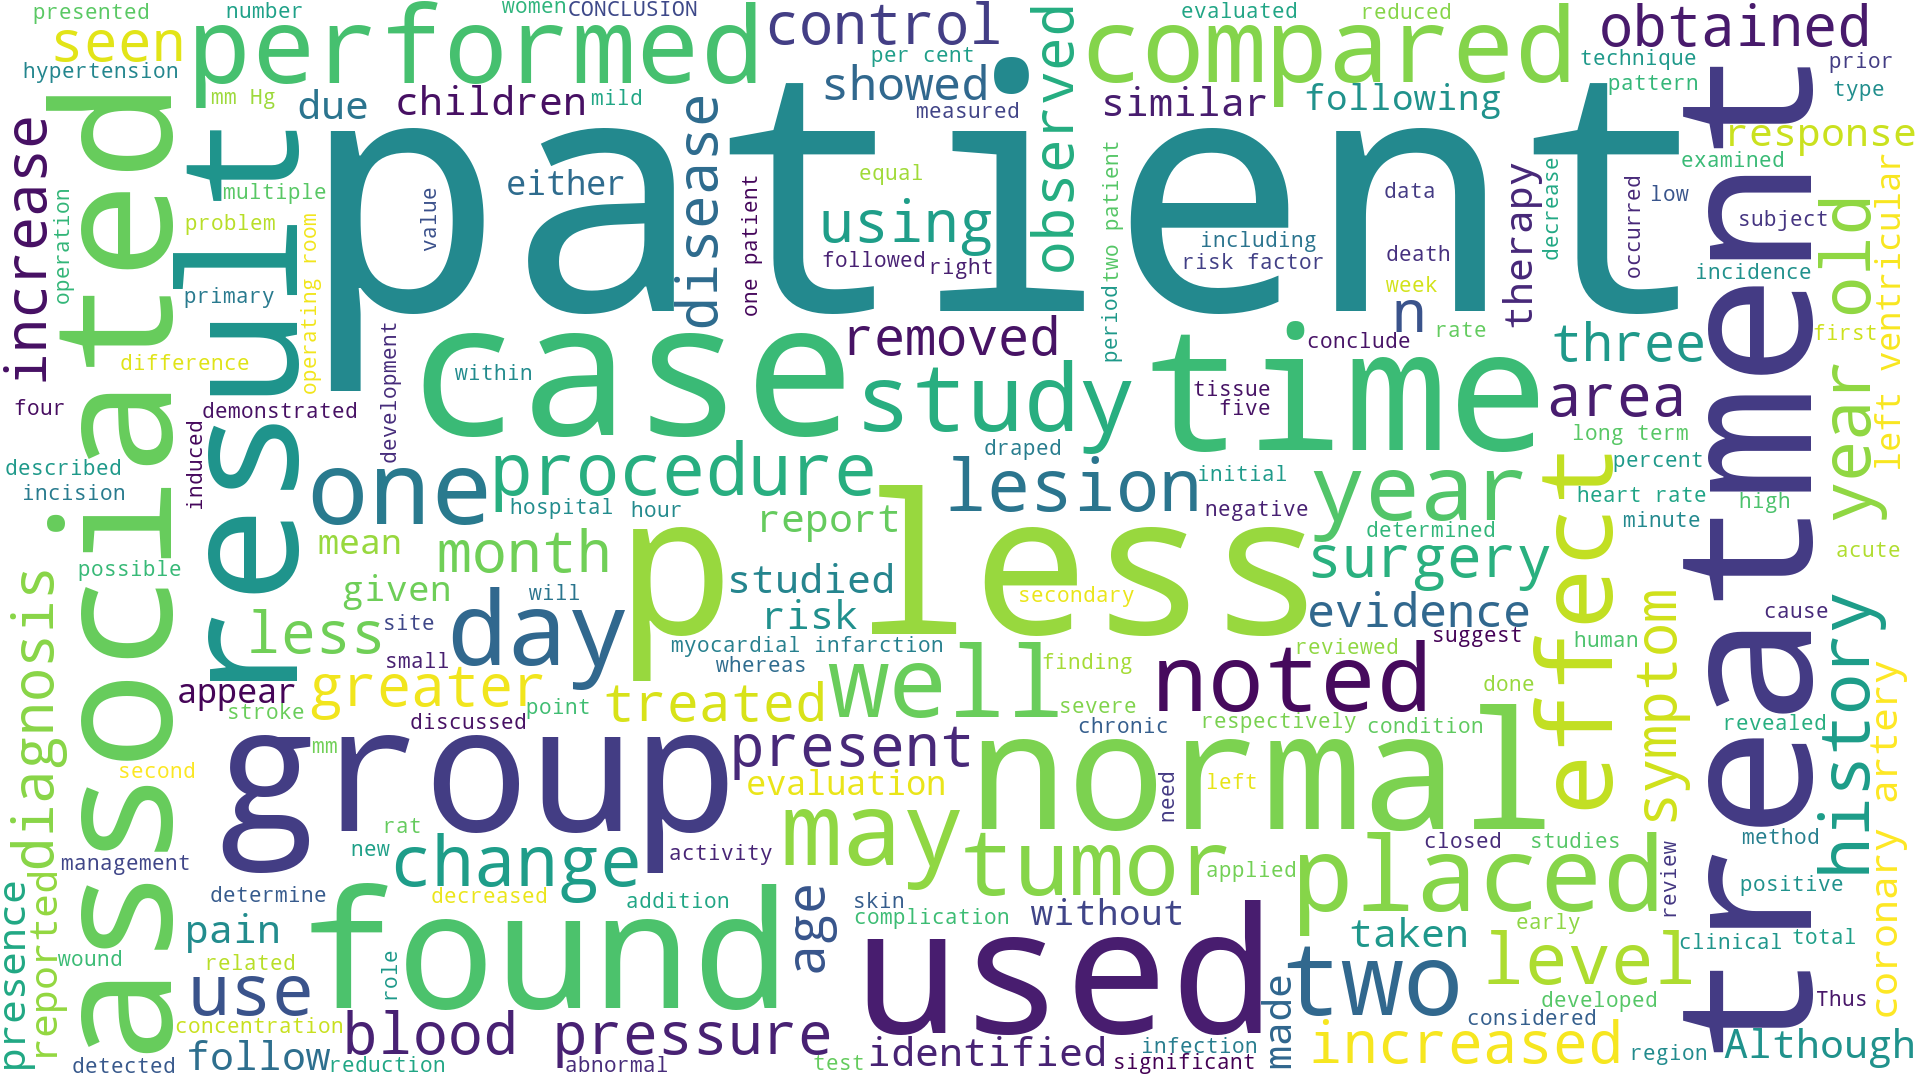
\includegraphics[width=.9\textwidth]{media/wordcloud_full_data.png}
	\caption{Wordcloud de todo el conjunto de datos}
	\label{fig:wordcloud}
\end{figure}

Se aprecia que las palabras más comunes son \textit{patient}, \textit{case}, o \textit{treatment}, junto con \textit{study} o \textit{performed}.

Disponiendo de este dataset, estamos listos para poder entrenar y ajustar nuestro modelo para que genere comentarios muy similares a los presentes en nuestro conjunto de datos.


\section{Resultados}

Habiendo preprocesado los datos, entrenado el modelo, guardado su estado y decidido el método de decodificación, estamos listos para poder generar comentarios. Se presentan aquí dos ejemplos generados al azar:

\begin{thm}
	\sffamily{
		Paediatric invasive immunosuppression (IPIS) in the treatment of recurrent kidney disease. Epidemiologic evidence suggests a association between immunosuppression and recurrence of recurrent kidney disease. Acute renal injury is a major risk factor for recurrent kidney disease. As the patient develops a family history of recurrence, his status will likely be monitored to determine whether he may benefit from continued immunosuppression.
	}
\end{thm}
\begin{thm}
	\sffamily{
		Predominant asymptomatic single cell carcinoma, melanoma, and cerebrovascular myopathy. The diagnosis of melanoma, cerebrovascular myopathy, and primary carcinoma requires extensive examination. Among these cancers, recurrent myopathy is a common occurrence. From 1980 to 1989, the incidence of melanoma, cerebrovascular myopathy, and secondary carcinoma increased from 8.5\% to 12.6\%.
	}
\end{thm}

Esto es solo una pequeña muestra. En la sección \ref{sec:comments} del apéndice se exponen alguno más, por si su inspección resultase de interés. 

Se puede apreciar que, a veces, los comentarios son muy cortos, como el comentario \ref{com:short}. En contadas ocasiones el generador ha devuelto una línea vacía. 

En ocasiones, los comentarios pueden no ser rigurosos médicamente hablando, pero esto, de cara al análisis de las herramientas disponibles para el procesamiento de los comentarios, no es estrictamente necesario. Necesitamos que los comentarios incluyan conceptos que sean importantes y destacables, como tipos de enfermedades, medicaciones, etc. De esta forma, podremos analizar cómo las herramientas detectan diferentes tipos de información y cómo de fiables son. 

Es por ello que poseer un generador de comentarios nos resulta conveniente, ya que se pueden considerar muchos más casos, prácticamente de forma ilimitada.

\subsection{Métricas y calidad de los comentarios}

Uno de los grandes retos de la creación de modelos de lenguaje, a parte de en sí ser el desarrollo de los mismos extremadamente complejo, es la creación de métricas de calidad de los resultados obtenidos.

Con modelos clásicos que trabajan con números, o incluso imágenes, existe una serie de herramientas que permiten ofrecer, de forma objetiva, rigurosa y consistente, un valor cuantitativo que mide la calidad de la salida de dicho modelo.

En los modelos de lenguaje, y más aún, en los modelos generativos, obtener un valor cuantitativo que evalúe la calidad de los comentarios generados es, más que complicado, subjetivo.

La pregunta que nos hacemos realmente es: ?`cómo de buenos son los comentarios generados? ?`Son comentarios coherentes? ?`Son comentarios rigurosos? ?`Cómo podemos evaluar de forma automática un conjunto de comentarios suficientemente representativo?

Para solucionar estos problemas, se han inventado algunas técnicas, anuque las más relevantes son la métrica BLEU \cite{BLEU} y la métrica Rouge \cite{lin2004rouge}.

\subsubsection{BLEU}
La métrica \textbf{B}i\textbf{L}ingual \textbf{E}valuation \textbf{U}nderstudy (BLEU) se ideó originalmente con objeto de evaluar traducciones automáticas. Dado un texto en un idioma y la traducción automática a otro, poder ofrecer un valor objetivo de cómo de bien se corresponden dichas oraciones. Esta tarea, como decíamos anteriormente, se compone de un importante carácter subjetivo, y es la razón por la que existen intérpretes y traductores que se encargan de este trabajo. La traducción de texto no es un mapeo directo de un conjunto de palabras de un idioma al de otro, ya que han de considerarse expresiones y valores culturales.

Dicho eso, disponer de, al menos, una medida que pueda servir de forma orientativa para evaluar la calidad de un traductor automático es, cuanto menos, conveniente.

El algoritmo en cuestión toma un conjunto de oraciones de referencia y otro conjunto de oraciones generadas que deseemos evaluar, y calcula un \textit{score} en función de cómo de probable es que una de las frases generadas pertenezca al conjunto de oraciones de referencia. Esta métrica también se utiliza extensivamente en evaluación de modelos generativos de lenguaje, como el nuestro, ya que la naturaleza de la evaluación se corresponde directamente con la nuestro caso de uso.


Para evaluar el modelo, tomamos 100 oraciones aleatorias de nuestro conjunto de datos, y generamos 100 oraciones con nuestro modelo. El valor obtenido es de 0.0036. 

Por referencia, la misma métrica nos ofrece un valor entre 0 y 1, donde un valor de 0 indica un nulo solapamiento del texto generado con el valor de referencia, y un valor cercano a 1 indica una buena traducción del texto dadas las referencias obtenidas.

Hay que tener en cuenta que es una medida de \textbf{solapamiento} especialmente diseñada para la evaluación de la traducción automática, por lo que nuestro valor cercano a 0 no necesariamente indica una mala calidad de la generación de los comentarios.

\subsubsection{Rouge}
La métrica Recall-Oriented Understudy for Gisting Evaluation (Rouge) funciona de una manera muy similar, calculando el solapamiento de las palabras en los textos a comparar y haciendo especial énfasis en las diferencias entre el número de tokens, ya que es una métrica especialmente diseñada para la evaluación de resúmenes. En esta métrica se obtuvo un valor de 0.0669, indicando un supuestamente mal resumen del texto. 

Como vemos, no son medidas muy útiles para nuestro propósito, pero lo cierto es que no existen muchas otras alternativas para la evaluación automática del lenguaje generativo libre, ya que es una tarea tan intrínsecamente subjetiva, como mencionábamos antes. Existe una opción en \cite{yuan2021bartscore}, pero el código no ha sido desvelado a día de hoy ya que continúa en desarrollo. 

Las medidas utilizadas anteriormente puede que no nos ofrezcan un valor objetivo de la calidad de los comentarios, pero sí nos ofrecen información acerca de su solapamiento, lo que nos lleva a la evaluación de similitud de los mismos.

\subsubsection{Similitud}
Esto nos lleva a otra métrica a utilizar: la distancia en los comentarios. Un factor que sí podemos determinar de forma sencilla es si los comentarios son muy similares entre sí. Idealmente, se desearía que el generador pudiera proporcionar comentarios que no estuvieran relacionados entre sí, ya que no se explora lo suficiente en el espacio de todas las posibles combinaciones de entidades que pudiésemos encontrar. En esencia, deseamos simular casos específicos y poco relacionados entre sí.

Para ello, podemos utilizar la medida de la distancia del coseno del valor TF-IDF mencionado en la sección \ref{sec:tfidf}. Calculando el valor TF-IDF de todos los comentarios generados y multiplicándolo por su traspuesta, generamos una matriz que nos define cómo de \textit{cerca} se encuentra cada comentario en el espacio latente. Podemos apreciar dicha matriz en la figura \ref{fig:conf-tfidf}. 

Se aprecia que la diagonal principal tiene un valor de 1, ya que se compara un comentario consigo mismo, por lo que la similitud es máxima (o la distancia 0).

Por lo general, todos los comentarios ofrecen valores de similitud muy bajos, que se intuye por la gran predominancia del color morado en la figura, que corresponde con valores cercanos a 0.

\begin{figure}[h]
	\centering
	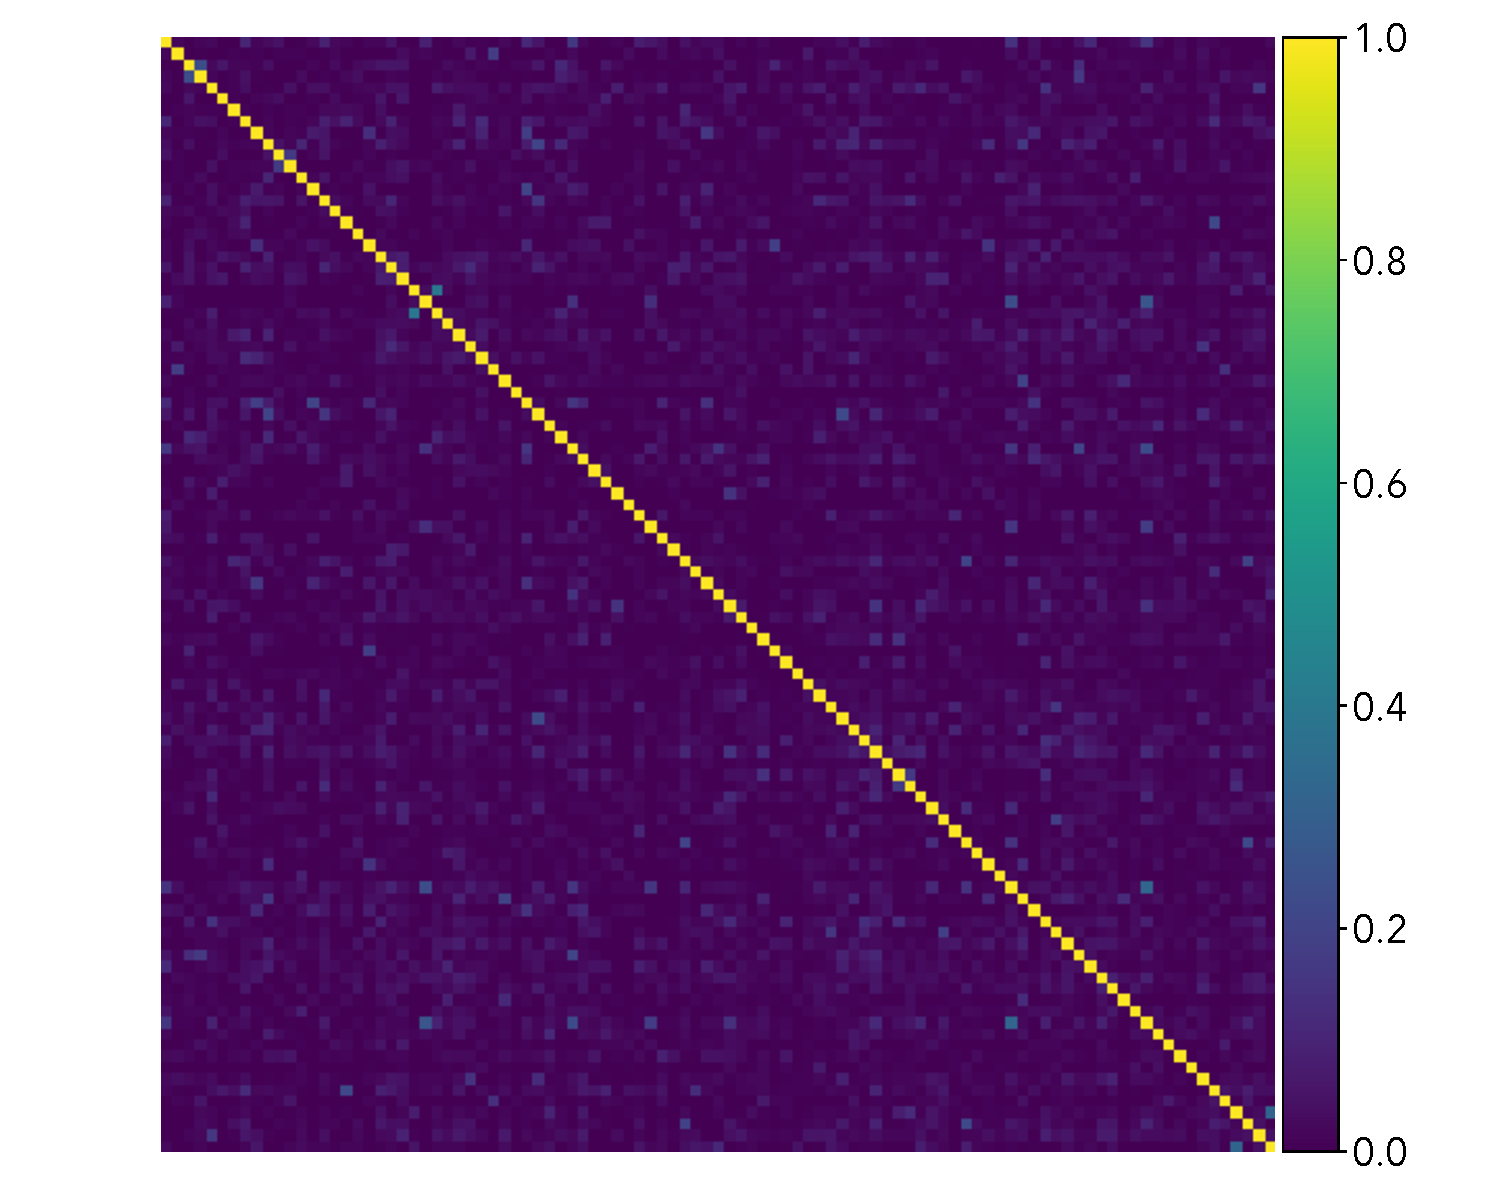
\includegraphics[width=.6\textwidth]{media/conf_matrix_tfidf.pdf}
	\caption{Matriz de comparativa de distancia de los 100 comentarios generados en todas las posibles combinaciones.}
	\label{fig:conf-tfidf}
\end{figure}



